\documentclass[09pt,letterpaper]{article}
\usepackage[lmargin=2.4in,rmargin=0.5in,tmargin=1.0in,bmargin=1.0in]{geometry}
\usepackage{notes}
\begin{document}


\begin{center}
\Large\textbf{1.2 – Growth/Decay Model, Solution Curves, and Direction Fields}\\
\normalsize (Sections 1.1.2, 1.1.3)
\end{center}



%-------------------------------------------------------------
\section{Verifying a Solution to a DE}

\subsection{Procedure}
To show that a function $x(t)$ solves a differential equation (DE), you must show that the left-hand side (LHS) equals the right-hand side (RHS) of the equation. If you are given an initial condition (IC), you must verify the equation as well. Here is an example.

\begin{example}[1]{
Suppose $k$ is a constant. Show that the function $x(t) = x_0 \,e^{kt}$ is a solution to the initial value problem
$$
\begin{dcases}
    x'=kx\\
    x(0)=x_0
\end{dcases}.
$$
}
\textbf{Step 1:} First, substitute $x$ into the LHS 
\begin{align*}
    \text{LHS} &= x'\\
            &=( x_0e^{kt})'\\
            &=k x_0e^{kt}.
\end{align*}
\textbf{Step 2:} Next, substitute $x$ into the RHS and show that it is identical to the LHS
\begin{align*}
    \text{RHS} &= kx\\ 
               &= k( x_0e^{kt})\\
               &= \text{LHS}\quad \checkmark
\end{align*}
\textbf{Step 3:} Lastly, verify the initial condition  
$$
x(0) = x_0 e^{0}=x_0\quad \checkmark 
$$
\end{example}

\subsection{Formula}
The IVP $x'=kx$ with $x(0)=x_0$ is an important equation that will arise frequently in this class. In the last example, we have established that 
$$
    x = x_0e^{kt}
$$
is the solution. You should get into the habit of using this result as a \textit{formula}. 

\begin{example}[2]{
Find the solution to the following DEs/IVPs. 
\begin{enumerate}
    \item[a)] $x'=7x$
    \item[b)] $x' = -3x$, $x(0)=10$.
\end{enumerate}
}
\begin{enumerate}
    \item[a)]
    The coefficient is $k=7$. This quantity becomes the coefficient in the exponent of the solution. The coefficient in front can just be $C$. The general solution is 
    $$
    \boxed{
        x(t) = C e^{7t}
    }
    $$
    \item[b)]
    The coefficient is $k=-3$, so the general solution is 
    $$
        x(t) = C e^{-3t}.
    $$
    We can apply the general solution and solve for $C$. That will give us the solution to the IVP:
    $$
        x(0)=10 =C, \;\implies \boxed{x(t)= 10e^{-3t}}
    $$
\end{enumerate}
\end{example}

% Now, for a small twist. Let's say you are given the solution containing unknown parameters. You can substitute the function into the DE to find the unknown values.
% \begin{example}[2]{
% Suppose the function
% $$
% x(t) = e^{at}
% $$
% is a solution to the DE
% $$
% x'' +6x = x'.
% $$
% What is (are) the value(s) of $a$? 
% }
% We can substitute the function into the DE: 
% \begin{align*}
%     x''+6x&=x'\\
%             (e^{at})'' + 6(e^{at})&=(e^{at})'\\
%             a^2 e^{at} + 6e^{at}&=a e^{at}\\
%             (a^2+6)e^{at}&=a e^{at}.
% \end{align*}
% We may divide both sides by $e^{at}$ since exponential functions are never zero:
% \begin{align*}
%     (a^2+6)\cancel{e^{at}} &= a \cancel{e^{at}}\\
%     a^2 + 6  &= a\\
%     a^2 - a + 6 &=0\\
%     (a-3)(a+2) &=0\\
%     \therefore a&=-2,3
% \end{align*}
% The values of $a$ are $-2$ and $3$.
% \end{example}

%-----------------------------------------------------
\section{Types of Solutions}

\subsection{General Solution}
Consider the DE 
$$x'=-kx$$ 
for $k>0$. Based on our formula, we know
$$ x(t) = C e^{-kt}$$
solves the equation. We call this the \textbf{general solution} because this one function captures every solution using an arbitrary constant $C$.

\subsection{Family of Solutions}
This function $x(t)=Ce^{-kt}$ also captures discrete solutions for each value of $C$. For instance, we can let $C=1, 0.5,-0.5,-1$, etc. This creates an infinite set of functions that are all solutions:
$$
\mathcal{F}=\{\ldots,-e^{-kt},-0.5e^{-kt},0.5e^{-kt},e^{-kt}\,\ldots\}
$$
We refer to this set $\mathcal{F}$ as a \textbf{family of solutions}. We can plot a few members of the family in one graph to visualize them. Here is an interesting fact: \textbf{a family of solutions can never intersect}.

\begin{figure}[H]
    \centering
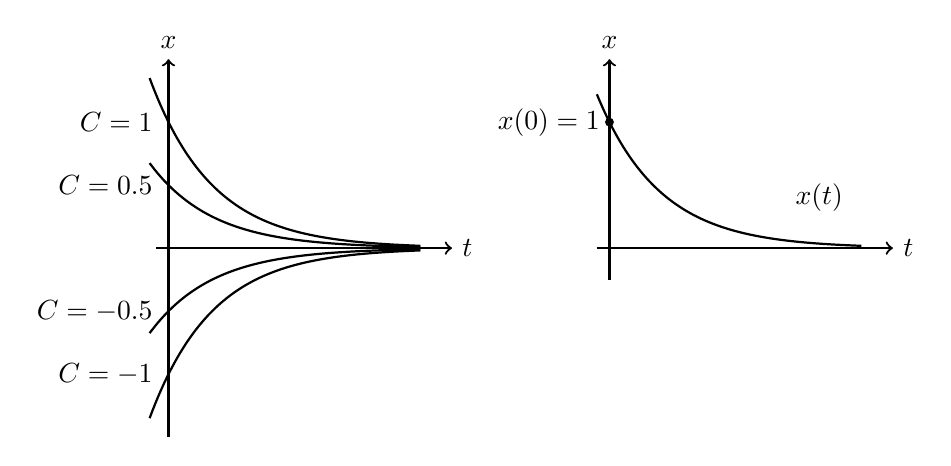
\begin{tikzpicture}[scale=0.8]
\begin{scope}
    % Axes
    \draw[->,thick] (-0.2,0) -- (4.5,0) node[right] {$t$};
    \draw[->,thick] (0,-3) -- (0,3) node[above] {$x$};

    % Curves x(t) = C e^{-t}
    \draw[thick,domain=-0.3:4,samples=100] plot (\x,{ 2*exp(-\x)});
    \draw[thick,domain=-0.3:4,samples=100] plot (\x,{ 1*exp(-\x)});
    \draw[thick,domain=-0.3:4,samples=100] plot (\x,{-1*exp(-\x)});
    \draw[thick,domain=-0.3:4,samples=100] plot (\x,{-2*exp(-\x)});

    % Labels
    \node[left] at (-0.1,2) {$C=1$};
    \node[left] at (-0.1,1) {$C=0.5$};
    \node[left] at (-0.1,-1) {$C=-0.5$};
    \node[left] at (-0.1,-2) {$C=-1$};
\end{scope}

% =======================
% RIGHT: Particular solution
% =======================
\begin{scope}[xshift=7cm]
    % Axes
    \draw[->,thick] (-0.2,0) -- (4.5,0) node[right] {$t$};
    \draw[->,thick] (0,-0.5) -- (0,3) node[above] {$x$};

    % Particular solution
    \draw[thick,domain=-0.2:4,samples=100] plot (\x,{ 2*exp(-\x)});

    % Initial condition point
    \fill (0,2) circle (2pt);
    \node[left] at (0,2) {$x(0)=1$};

    % Label
    \node[right] at (2.8,0.8) {$x(t)$};
\end{scope}
\end{tikzpicture}\caption{The left figure shows a family of solutions to $x'=-kx$. The right figure shows the one particular solution corresponding to an initial condition $x(0)=1$.}
\end{figure}

\subsection{Particular Solution}
Consider the initial value problem (IVP)
\[
\begin{dcases}
x' = -kx,\\
x(0) = 1.
\end{dcases}
\]
Using the initial condition (IC) $x(0)=1$, we may solve for the value of $C$:
\[
1 = Ce^{-k(0)}=C,
\]
so the solution is 
\[
x(t) = e ^{-kt}.
\]
We call this a \textbf{particular solution} of $x'=-kx$ because it satisfies a particular IC. The IC $x(0)=1$ corresponds to the point $(0,1)$ on the $tx$-plane. Fact: \textbf{the particular solution is the one member of the family passing through the point $(0,1)$.}


%-------------------------------------------------------------
\section{The Growth/Decay Model}
This section is about equations of the form $x' = kx$. 

\subsection{Growth Model}
Suppose $x(t)$ represents the quantity of something at time $t$. Then the derivative $x'$ represents its rate of change. Suppose that the rate of change of $x(t)$ is proportional to the amount $x(t)$ itself:
\[
x' \propto x.
\]
Introducing a constant of proportionality $k>0$, we write
\[
x' = kx.
\]
This equation is called the \textbf{growth model}.
If $x$ is small, then $x'$ is also small.
If $x$ is large, then $x'$ is also large.
In other words, the more you have, the faster the quantity grows.

\subsection{Exponential Growth}
The model $x'=kx$ is appropriate for:
\begin{itemize}
    \item $x(t)=$ amount of money in a bank account earning compound interest,
    \item $x(t)=$ population of bacteria reproducing freely,
    \item $x(t)=$ the size of a snowball rolling down a snowy hill.
\end{itemize}
In each case, the quantity $x(t)$ grows slowly at first, but then speeds up as the $x(t)$ itself becomes large. This leads to rapid accumulation due to a snowball effect. The way $x(t)$ increases with respect to time is called \textbf{exponential growth}.

% \begin{figure}[H]
%     \centering
% \begin{tikzpicture}[scale=0.8]
% \begin{scope}
%     % Axes
%     \draw[->,thick] (-0.2,0) -- (4.5,0) node[right] {$t$};
%     \draw[->,thick] (0,-0.1) -- (0,3) node[above] {$x$};
%     % Curves x(t) = C e^{-t}
%     \draw[thick,domain=0:4,samples=100] plot (\x,{ 1*exp(0.3*\x)});
%     % Labels
%     \node[left] at (-0.1,1) {$x(0)=x_0$};
% \end{scope}
% \end{tikzpicture}
%     \caption{Growth model solution.}
% \end{figure}

\subsection{Word Problem}
We can use this knowledge about the growth model to answer some questions. The steps are:
\begin{enumerate}
    \item Set up the model. 
    \item Solve the IVP. 
    \item Use the solution to answer the question.
\end{enumerate}
Here is an example.

\begin{example}[3]{
Suppose \$1000 is deposited into a bank account that earns interest continuously at an annual rate of $5\%$. Determine how long it takes for the balance to double.
}

\begin{enumerate}
\item \textbf{Set up the model.} Let $x(t)$ be the balance in dollars after $t$ years. The initial balance is \$1000 so we let $x(0)=1000$. Since the growth rate is $r=5\% = 0.05$, our model is
\[
\begin{dcases}
x' = 0.05x,\\
x(0)= 1000.
\end{dcases}
\]
\item \textbf{Solve the IVP.} Any DE of the form $x'=kx$ always has the same form. We may write the solution using the formula
\[
x(t) = x_0 e^{kt} =1000\,e^{0.05t}.
\]
\item \textbf{Use the solution.} Set $x(t)=2000$ and solve for $t$:
\begin{align*}
2000 &= 1000 e^{0.05t} \\
2 &= e^{0.05t} \\
\ln 2 &= 0.05t \\
t &= \frac{\ln 2}{0.05} \approx 13.86.
\end{align*}
Final answer: it takes $\boxed{t \approx 13.9 \text{ years}}$ for the bank balance to grow from $\$1000$ to $\$2000$.
\end{enumerate}
\end{example}


\subsection{Decay Model}

Again, let's suppose $x(t)$ represents the amount of some material at time $t$. If the derivative is negative ($x'<0$), then that means the amount is \textit{decreasing} over time. If the rate of decrease is proportional to the remaining amount, then we write
\[
x' \propto -x,
\]
or rather
\[
x' = -kx,
\]
where $k>0$. The parameter $k$ represents the percentage amount lost after each time step. This differential equation is called the \textbf{decay model}.  This DE can model:
\begin{itemize}
    \item radioactive decay of a substance,
    \item cooling of a hot object in a cooler environment,
    \item discharge of a capacitor.
\end{itemize}
In the decay model, the quantity decreases quickly at first, but the rate of decay slows as less material remains. 

Here is a quick example. Let's say a rubber ball bounces back up $\%50$ of its height from the previous bounce. If it's dropped from 1 meter, then it bounces up to $0.5$ meters, $0.25$ meters, etc. If $x$ is the bounce height and $t$ is the number of bounces, we may write
$$
x' = -0.5 x,\quad x(0)=1
$$
to model the ball.


%-----------------------------------------------------
\section{Geometric Approach}
We may gain insight into the solution of a first-order DE without explicitly solving the equation. In this section, we focus on understanding the qualitative behavior of solution curves from a geometric perspective.

\subsection{Interpreting IVPs}

Consider the first-order IVP
$$
\frac{dx}{dt} = f(t,x),\quad x(t_0)=x_0,
$$
where the goal is to find the unknown function $x(t)$. Let's begin by establishing a mental picture of the solution. You can interpret the solution as a curve existing in the $\mathbf{tx}$-\textbf{plane}. We refer to the plotted function as the \textbf{solution curve} or \textbf{integral curve}. 

There are three important aspects of IVPs:
\begin{enumerate}
    \item \textbf{Slope} $\mathbf{\tfrac{dx}{dt}}$: the slope tells us the "steepness" of the line tangent to the solution curve.  
    \item \textbf{Formula} $\mathbf{f(t,x)}$: the formula is effectively a function that allows us to calculate the slope of the solution at any point in the $(t,x)$ plane.
    \item \textbf{Initial Condition} $\mathbf{x(t_0)=x_0}$: the IC tells us that the curve must pass through the point $(t_0, x_0)$. 
\end{enumerate}
The figure below illustrates these ideas geometrically. We may obtain a rough idea of the solution curve without solving anything.

\begin{figure}[H]
    \centering
    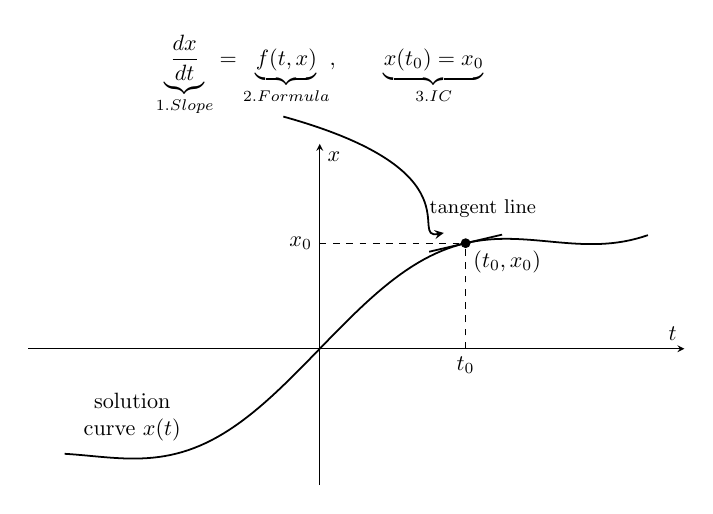
\begin{tikzpicture}[
        scale=0.8,
        >=stealth,
        declare function={
            k = 1.2;
            tzero = 2.0;
            xfun(\t) = k*sin(deg(\t)) + \t;
            slope(\t) = k*cos(deg(\t)) + 1;
            xzero = xfun(tzero);
        }
    ]
    
    \begin{axis}[
        width=12cm,
        height=7cm,
        axis lines=center,
        xmin=-4, xmax=5,
        ymin=-4, ymax=6,
        xlabel={$t$},
        ylabel={$x$},
        xtick=\empty,
        ytick=\empty,
        clip=false,
    ]
    
    % solution curve x(t)
    \addplot[
        thick,
        domain=-3.5:4.5,
        samples=100,
    ]
    {xfun(x)};
    
    % point (t0,x0)
    \addplot[
        only marks,
        mark=*,
        mark size=2pt,
    ]
    coordinates {(tzero,xzero)};
    
    % dashed guides
    \draw[dashed] (axis cs:tzero,0) -- (axis cs:tzero,xzero);
    \draw[dashed] (axis cs:0,xzero) -- (axis cs:tzero,xzero);
    
    \node[below] at (axis cs:tzero,0) {$t_0$};
    \node[left] at (axis cs:0,xzero) {$x_0$};
    \node[below right] at (axis cs:tzero,xzero) {$(t_0,x_0)$};
    
    % tangent line at t0
    \addplot[
        thick,
        domain=1.5:2.5,
        samples=2,
    ]
    {xzero + slope(tzero)*(x-tzero)};

    % tangent 
    \node[align=center,right] at (axis cs:1.4,4.1)
    {\small tangent line};
    
    % solution curve label
    \node[align=center,left] at (axis cs:-1.8,-2.0)
    {solution\\curve $x(t)$};
    
    
    % equation above plot
    \node[align=center] at (axis cs:0,8.0)
    {$\displaystyle
    \underbrace{\frac{dx}{dt}}_{\text{1. Slope}}
    =
    \underbrace{f(t,x)}_{\text{2. Formula}},
    \qquad
    \underbrace{
    x(t_0)=x_0}_{\text{3. IC}}
    $};
    
    % arrow from f(t,x) idea to tangent
    \draw[->,thick]
    (axis cs:-0.5,6.8)
    .. controls (axis cs:2.2,5.2) and (axis cs:1.2,3.2)
    .. (axis cs:tzero-0.3,xzero+0.3);
    
    
    \end{axis}
    \end{tikzpicture}
    \caption{Think of first-order IVPs as a task to to find a solution curve $x(t)$ going through the point $(t_0,x_0)$ which obeys a specified slope formula $f(t,x)$.}
\end{figure}

% ---------------------------------------------

\subsection{Slope Analysis}
There are two interesting slopes: $x'=0$ and $x'=\pm\infty$. If a certain combination of $(t,x)$ forces $x'=f(t,x)$ to be zero, then we know there's a \textit{horizontal tangent} located at $(t,x)$. If the slope is $\pm\infty$ (in the limit), then there must be a vertical tangent. Let's see an example. 


\begin{example}[4]{

Consider the IVP
\[
x'=-x^2, \quad x(2)=1.
\]
What can you infer about the solution curve? Assume $x>0$. 
}
\vspace{1em}

First of all, we know the solution goes through the point $(2,1)$. Next, notice that since
\[
x'=-x^2 \leq 0
\]
for every value of $x$, the curve must be \textit{monotonically decreasing}. At the point $(2,1)$, the slope is
\[
x' = -(1)^2 = -1.
\]
Thus, the tangent line at $x=1$ has a slope of $-1$.

Next, let us examine how the slope behaves for large values of $x$. Since
\[
\lim_{x\to\infty} -x^2 = -\infty,
\]
the slope becomes extremely negative when $x$ is large. As we move \emph{north} from $(2,1)$, the curve becomes a vertical asymptote. Since
\[
\lim_{x\to 0^+} -x^2 = 0,
\]
the curve should flatten out as we move \emph{south} from $(2,1)$ towards the $t$-axis. The general solution is
\[
x(t)=\frac{1}{t+C},
\]
and is plotted below. The function curve of the function is as predicted.

\begin{figure}[H]
\centering
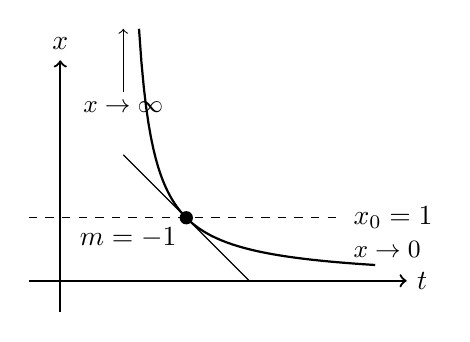
\begin{tikzpicture}[scale=0.8]

% Axes
\draw[->,thick] (-0.5,0) -- (5.5,0) node[right] {$t$};
\draw[->,thick] (0,-0.5) -- (0,3.5) node[above] {$x$};

% solution curves x(t) = 1/(t-1)
% \draw[thick,dashed,domain=-2.4:0.55,samples=100] plot (\x,{1/(\x-1)});
\draw[thick,,domain=1.25:5,samples=100] plot (\x,{1/(\x-1)});


% Vertical asymptotes
\draw[->] (1,3) -- (1,4);
\node[below] at (1,3) {\small $x\to\infty$};

% At x0 = 1
\fill (2,1) circle (3pt);
\draw[dashed] (-0.5,1) -- (4.5,1);
\node[right] at (4.5,1) {$x_0=1$};
\draw (1,2) -- (3,0);
\node[below left] at (2,1) {$m=-1$};

% Horizontal behavior
% \draw[->,thick] (4.5,0.5) -- (5.2,0.5);
\node[right] at (4.5,0.5) {\small $x\to 0$};

\end{tikzpicture}
\caption{The general solution to $x'=-x^2$ is $x(t)=\frac{1}{t+C}$. The plot above shows the particular solution $x(t) = \frac{1}{t-1}$.}
\end{figure}
\end{example}


\subsection{Direction Fields}

In the DE
\[
x' = f(t,x)
\]
the function $f(t,x)$ gives us a formula for the slope at any point $(t,x)$. We may populate an entire $tx$-plane full of slopes calculated at their respective coordinates. The resulting picture is called the \textbf{direction field}.

For instance, consider the DE
$$
x' = f(t,x)= t^2 - x.
$$
Let's choose the point $(-1,2)$ ($t=-1$ and $x=2$). Since $f(-1,2) = (-1)^2-2= -1$, we draw a line with slope $m=-1$ at the coordinate $(-1,2)$. The figure below shows the direction field. 

\begin{figure}[H]
    \centering
    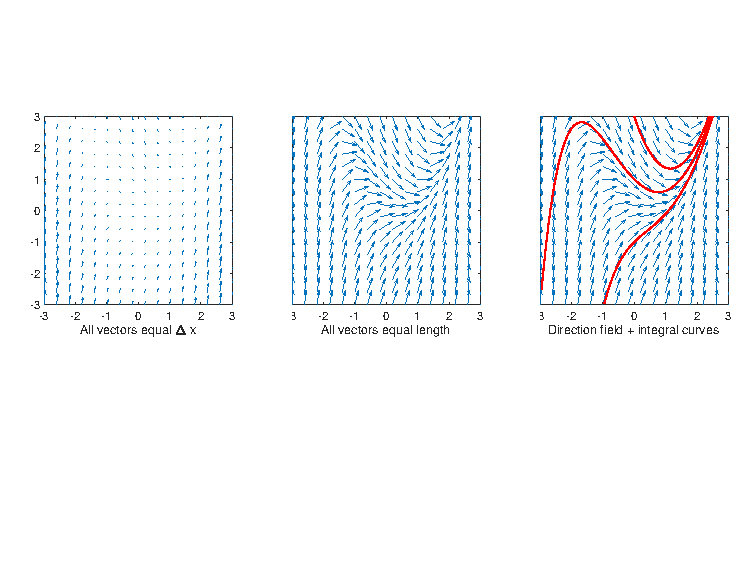
\includegraphics[width=1.0\linewidth]{figs/dirfield2.pdf}
    \caption{The figures above show direction fields for the equation $x' = t^2-x$. }
\end{figure}

\subsection{Solution Curves on Direction Fields}
What makes direction fields so powerful? \textbf{They let us sketch solutions to IVPs for any IC.}
The figure below shows the direction field for the IVP
$$
x' = t + \sin(x), \quad x(t_0)=x_0.
$$
The red curves are all solutions to the DE corresponding to different initial conditions.  To obtain the solution curve, 
\begin{enumerate}
    \item draw a dot at the point $(t_0,x_0)$. 
    \item trace a path in the direction of the slope
    \item stop when you encounter a new slope
    \item return to step 2
\end{enumerate}

\begin{figure}[H]
\centering
    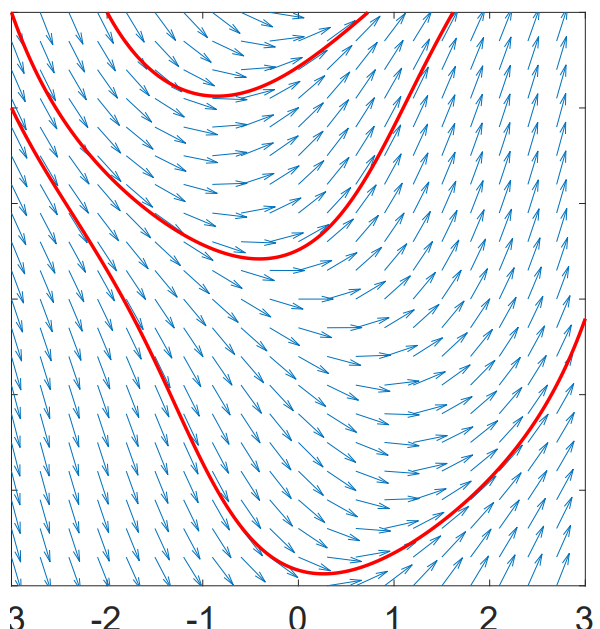
\includegraphics[width=0.4\linewidth]{figs/df2.png}
    \caption{These figures show how solution curves can be drawn on direction fields. This is example 1 on the syllabus page \texttt{https://math.unm.edu/\~{}nitsche/courses/316/}. You are encouraged to see the other five examples.}    
\end{figure}



% --------------------------------------------------

\section{Graphing by Superposition}
This section is about plotting sums of functions such as $y_1=x^2$ plus $y_2=\cos x$.

\subsection{Common Functions}
You are expected to know how to sketch the following common functions by hand:
\begin{multicols}{2}
\begin{itemize}
    \item $y=k$ (constant)
    \item $y=x$
    \item $y=x^2$
    \item $y=x^3$
    \item $y=\sqrt{x}$
    \item $y=1/x$
    \item $y=1/x^2$
    \item $y=e^x$
    \item $y=e^{-x}$
    \item $y=\cos(x)$
    \item $y=\sin(x)$
\end{itemize}
\end{multicols}

\noindent These functions are less common, but they are relevant to this course
\begin{itemize}
    \item $y=\frac{1}{1+e^{-x}}$ \quad  (S-shaped sigmoid function)
    \item $y=\tan^{-1}(x)$ \quad (looks like an S with asymptotes at $\pm\pi/2$)
    \item $y=\cosh (x)$ \quad (looks like $x^2+1$)
    \item $y=\sinh(x)$ \quad (looks like $x^3$)
\end{itemize}

\subsection{Graphing Technique}
\textbf{Graphing by superposition} is a technique that allows you to sketch the sum of two functions such as $f = 1 + \sin x$. The idea is to sketch the two pieces of the function together on one graph. Then you sketch the sum by combining the elevations of the two functions. When you add two positive functions, the sum is shifted upwards. When you add two negative functions, the sum is shifted downwards. 

\begin{example}[5]{
Sketch $y = x+ \sin x$ by hand. 
}    
Begin by sketching $y_1=x$ and $y_2 = \sin x$ in dashed lines on the same graph. Then plot the sum by combining the heights of both functions. Since $y=x$ is negative for $x<0$, the sine wave is shifted down. Similarly, $y=x$ is positive for $x>0$, so the sine wave is shifted up.
\begin{figure}[H]
\centering
\begin{tikzpicture}[scale=0.45]
% Axes
\draw[->,thick] (-6,0)--(6,0) node[right]{$x$};
\draw[->,thick] (0,-4)--(0,4) node[above]{$y$};

% f1 = x (red dashed)
\draw[red,dashed,thick,domain=-5:0,samples=100]
    plot(\x,\x);
% f1 = x (green dashed)
\draw[dgreen,dashed,thick,domain=0:5,samples=100]
    plot(\x,\x);
\node[right] at (4,4) {$y=x$};

% f2 = sin x (dashed)
\draw[dashed,thick,domain=-5:5,samples=100]
    plot(\x,{sin(\x r)});
\node[right] at (4,-2) {$y=\sin x$};

% f = x + sin x (solid)
% \draw[thick,domain=-5:5,samples=200]
%     plot(\x,{\x + sin(\x r)});
% \node[right] at (4,3) {$y=x+\sin x$};
\end{tikzpicture}
%-------------------------------------
\begin{tikzpicture}[scale=0.45]
% Axes
\draw[->,thick] (-6,0)--(6,0) node[right]{$x$};
\draw[->,thick] (0,-4)--(0,4) node[above]{$y$};

% f1 = x (red dashed)
\draw[red,dashed,thick,domain=-5:0,samples=100]
    plot(\x,\x);
% f1 = x (green dashed)
\draw[dgreen,dashed,thick,domain=0:5,samples=100]
    plot(\x,\x);
% f2 = sin x (dashed)
\draw[dashed,thick,domain=-5:5,samples=100]
    plot(\x,{sin(\x r)});
% f = x + sin x (solid)
\draw[thick,domain=-5:5,samples=200]
    plot(\x,{\x + sin(\x r)});
\node[right] at (1,4) {\small shift up};
\node[right] at (-4,-4) {\small shift down};

\end{tikzpicture}
\caption{Graphing by superposition: the dashed curves are $y=x$ and $y=\sin x$, and the solid curve is their sum $y=x+\sin x$.}
\end{figure}
\end{example}

% \subsection{Using Desmos}

% Sketching transformations of functions is a skill that develops with practice, so it is normal for graphing unfamiliar functions to feel difficult at first. Graphing software can help build intuition by allowing us to visualize how different pieces of a function interact. One particularly useful free tool is 
% \[
% \texttt{desmos.com}.
% \]
% We will briefly discuss how Desmos can help us sketch functions through superposition.

% Consider the function
% \[
% f(x)=x+\frac1x.
% \]
% Rather than trying to understand the entire function at once, we can break it into simpler pieces:
% \[
% f_1(x)=x,
% \qquad
% f_2(x)=\frac1x.
% \]
% In the first two lines of Desmos, create the functions $f_1$ and $f_2$. You can adjust the color, opacity, thickness, and line style of these functions by long-pressing the icon on the left. For example, you can make the graph of $f_1(x)$ thin, dashed, and red.  On the third line plot $f_1(x)+f_2(x)$. The figure below shows the complete picture with $f=x+\frac1x$ plotted in black. 

% \begin{figure}[H]
%     \centering
%     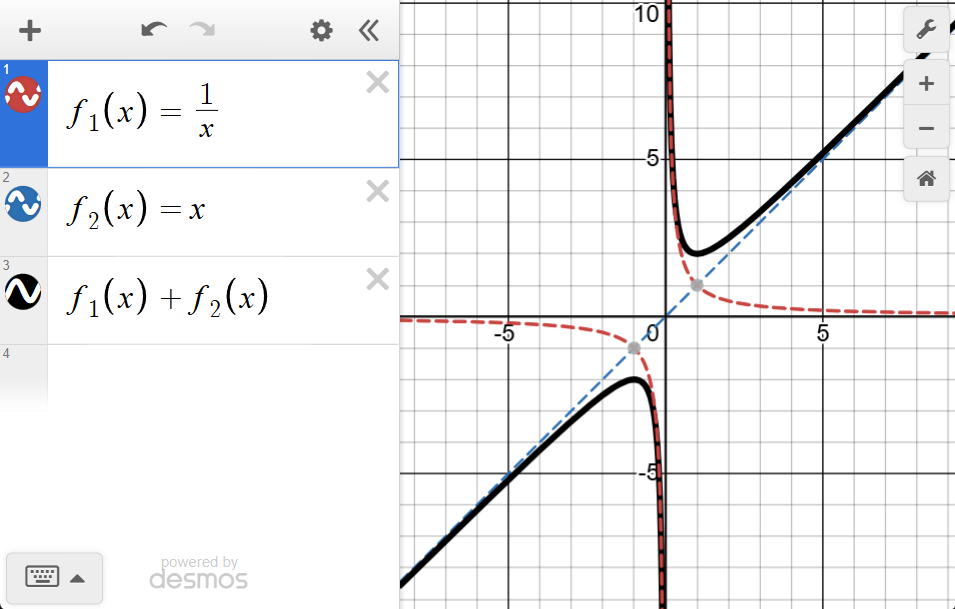
\includegraphics[width=0.9\linewidth]{figs/desmos.png}
%     \caption{This is a screenshot from \texttt{desmos.com/calculator}. The sum $x+\frac1x$ is plotted in the thick, solid, black line.}
% \end{figure}

% \noindent It is important to be able to make sense of the plot because you will not be able to use graphing tools on exams. You should consider the regions $x>0$ and $x<0$ separately.
% \begin{itemize}
%     \item For $x>0$, both $x$ and $\frac1x$ are positive. 
%     Thus their sum is also positive. 
    
%     Near $x=0^+$, the term $\frac1x$ becomes very large, causing the graph to shoot upward. For large positive $x$, the linear term $x$ dominates, so the graph begins to resemble the line $y=x$.

%     \item For $x<0$, both $x$ and $\frac1x$ are negative. 
%     Their sum is therefore negative as well.
    
%     Near $x=0^-$, the term $\frac1x$ becomes very large in magnitude and negative, causing the graph to plunge downward. For large negative $x$, the graph again behaves approximately like the line $y=x$.
% \end{itemize}


% \begin{figure}[H]
% \centering
% \begin{tikzpicture}[scale=0.8]

% % Axes
% \draw[->,thick] (-6,0)--(6,0) node[right]{$x$};
% \draw[->,thick] (0,-6)--(0,6) node[above]{$y$};

% % Vertical asymptote
% \draw[dashed] (0,-6)--(0,6);
% \node[above right] at (0,5) {$x=0$};

% % f1 = x (dashed)
% \draw[dashed,thick,domain=-5:-0.3,samples=100]
%     plot(\x,\x);
% \draw[dashed,thick,domain=0.3:5,samples=100]
%     plot(\x,\x);
% \node[right] at (4,4) {$y=x$};

% % f2 = 1/x (dashed)
% \draw[dashed,thick,domain=-5:-0.3,samples=100]
%     plot(\x,{1/\x});
% \draw[dashed,thick,domain=0.3:5,samples=100]
%     plot(\x,{1/\x});
% \node[right] at (2,1) {$y=\tfrac1x$};

% % f = x + 1/x (solid)
% \draw[thick,domain=-5:-0.3,samples=200]
%     plot(\x,{\x + 1/\x});
% \draw[thick,domain=0.3:5,samples=200]
%     plot(\x,{\x + 1/\x});
% \node[right] at (2.5,3) {$y=x+\tfrac1x$};

% \end{tikzpicture}
% \caption{Graphing by superposition: dashed curves show $y=x$ and $y=\tfrac1x$. Their sum $y=x+\tfrac1x$ is V-shaped on each side of the vertical asymptote.}
% \end{figure}



\end{document}
